%Preamble
\documentclass[12pt]{article}\usepackage[]{graphicx}\usepackage[]{color}
%% maxwidth is the original width if it is less than linewidth
%% otherwise use linewidth (to make sure the graphics do not exceed the margin)
\makeatletter
\def\maxwidth{ %
  \ifdim\Gin@nat@width>\linewidth
    \linewidth
  \else
    \Gin@nat@width
  \fi
}
\makeatother

\definecolor{fgcolor}{rgb}{0.345, 0.345, 0.345}
\newcommand{\hlnum}[1]{\textcolor[rgb]{0.686,0.059,0.569}{#1}}%
\newcommand{\hlstr}[1]{\textcolor[rgb]{0.192,0.494,0.8}{#1}}%
\newcommand{\hlcom}[1]{\textcolor[rgb]{0.678,0.584,0.686}{\textit{#1}}}%
\newcommand{\hlopt}[1]{\textcolor[rgb]{0,0,0}{#1}}%
\newcommand{\hlstd}[1]{\textcolor[rgb]{0.345,0.345,0.345}{#1}}%
\newcommand{\hlkwa}[1]{\textcolor[rgb]{0.161,0.373,0.58}{\textbf{#1}}}%
\newcommand{\hlkwb}[1]{\textcolor[rgb]{0.69,0.353,0.396}{#1}}%
\newcommand{\hlkwc}[1]{\textcolor[rgb]{0.333,0.667,0.333}{#1}}%
\newcommand{\hlkwd}[1]{\textcolor[rgb]{0.737,0.353,0.396}{\textbf{#1}}}%
\let\hlipl\hlkwb

\usepackage{framed}
\makeatletter
\newenvironment{kframe}{%
 \def\at@end@of@kframe{}%
 \ifinner\ifhmode%
  \def\at@end@of@kframe{\end{minipage}}%
  \begin{minipage}{\columnwidth}%
 \fi\fi%
 \def\FrameCommand##1{\hskip\@totalleftmargin \hskip-\fboxsep
 \colorbox{shadecolor}{##1}\hskip-\fboxsep
     % There is no \\@totalrightmargin, so:
     \hskip-\linewidth \hskip-\@totalleftmargin \hskip\columnwidth}%
 \MakeFramed {\advance\hsize-\width
   \@totalleftmargin\z@ \linewidth\hsize
   \@setminipage}}%
 {\par\unskip\endMakeFramed%
 \at@end@of@kframe}
\makeatother

\definecolor{shadecolor}{rgb}{.97, .97, .97}
\definecolor{messagecolor}{rgb}{0, 0, 0}
\definecolor{warningcolor}{rgb}{1, 0, 1}
\definecolor{errorcolor}{rgb}{1, 0, 0}
\newenvironment{knitrout}{}{} % an empty environment to be redefined in TeX

\usepackage{alltt}
\usepackage{scrtime} % for \thistime (this package MUST be listed first!)
\usepackage[margin=1in]{geometry}
\usepackage{graphics,graphicx}
\usepackage{placeins}
\usepackage[displaymath, mathlines]{lineno}
\usepackage{color}
\definecolor{aqua}{RGB}{0, 128, 225}
\usepackage[colorlinks=true,citecolor=aqua,linkcolor=aqua,urlcolor=aqua]{hyperref}
%For Math stuff
\usepackage{amsmath} % essential for cases environment
\usepackage{amsthm} % for theorems and proofs
\usepackage{amsfonts, array, siunitx} % mathbb
\usepackage{animate}
\usepackage{tikz}
\usetikzlibrary{shapes.geometric, arrows}
%Referenes
\usepackage[natbib=true,
            style=nature,
            citestyle=authoryear,
            backend=biber,
            useprefix=true]{biblatex}
\addbibresource{./plagueDoctors.bib}
%FANCY HEADER AND FOOTER STUFF
\usepackage{fancyhdr,lastpage}
\pagestyle{fancy}
\fancyhf{} % clear all header and footer parameters
%%%\lhead{Student Name: \theblank{4cm}}
%%%\chead{}
%%%\rhead{Student Number: \theblank{3cm}}
%%%\lfoot{\small\bfseries\ifnum\thepage<\pageref{LastPage}{CONTINUED\\on next page}\else{LAST PAGE}\fi}
\lfoot{}
\cfoot{{\small\bfseries Page \thepage\ of \pageref{LastPage}}}
\rfoot{}
\renewcommand\headrulewidth{0pt} % Removes funny header line
\IfFileExists{upquote.sty}{\usepackage{upquote}}{}
\begin{document}
%Title
\title{Examining Control Strategies for Cholera Incorporating Spatial Dynamics}
\author{
\underline{\emph{Group Name}}: \texttt{{\color{blue}The Plague Doctors}}\\\\
\underline{\emph{Group Members}}:\\
         Sid Reed\ :\ {\color{blue}reeds4@mcmaster.ca}\\
         Daniel Segura\ :\ {\color{blue}segurad@mcmaster.ca}\\
         Jessa Mallare\ :\ {\color{blue}mallarej@mcmaster.ca}\\
         Aref Jadda\ :\ {\color{blue}hossesa@mcmaster.ca}\\
}
\date{\today\ @ \thistime}
\maketitle
%due date %\bigskip
%\noindent
%This assignment is {\bfseries\color{red} due in class} on \textcolor{red}{\bf Wednesday March 27 2019 at 10:30am}.
%\bigskip

\linenumbers

\begin{abstract}
    Cholera has a significant impact on public health, especially in areas with poor water sanitation, with infections estimated to affect between 1.3 and 4 million people annually \citep{link18}.
    Many people globally still lack proper infrastructure or access to clean water\citep{link19}.
    While vaccines and antibiotics exist, vaccination can be difficult to achieve at necessary levels for stopping an epidemic and widespread antibiotic usage contributes to the development of antibiotic resistance.
    Considering the spatial dynamics of water sanitation, antibiotic usage and vaccination are important for creating the most effective and efficient treatment regime in preventing cholera epidemics
\end{abstract}

\clearpage
\tableofcontents
\clearpage

%Sections
\section{Introduction}

\subsection{Biology of Cholera}
Although it is listed as one of the oldest known diseases, cholera remains a major public health concern in areas with poor water sanitation with an estimated 1.3--4 million cases every year \citep{link18}.
Cholera is an infectious disease caused by the bacterium \textit{Vibrio cholerae}.
The bacterium survives and reproduces in aquatic environments, and is capable of colonizing small intestines \citep{link8}.
The disease is not airborne, but can be transmitted through contaminated food or water and can survive in some aquatic environments from months to years \citep{link9}.
The bacterium produces enterotoxins responsible for the symptoms of cholera infection which are severe diarrhea, vomiting and nausea \citep{link11}.
%Approximately only one in ten people infected develop symptoms, and if not treated urgently, these symptoms can lead to severe dehydration.
Dehydration thickens the blood, causing circulation problems that can lead to death within a few hours.
Since dehydration is the main problem, rehydration with clean water and minerals (such as oral rehydration salts (ORS) packages) is the most effective treatment \citep{link18}.
Current improvements in public health and sanitation largely decrease the likelihood of a cholera outbreak \citep{link18}.\par
Four major outbreaks of cholera in the 19th century devastated the London population, resulting in tens of thousands of deaths.
One of the early theories believed to be the cause of spread of cholera was the Miasma theory, suggesting that cholera is an airborne disease and that impurities in the air induced the spread \citep{link1}.
Thus, the suggested solution in 1848 was to discard the contents of cesspools and raw sewage pits into the River Thames.
Since Thames was the drinking source of many, the misunderstanding about the method of transmission resulted in heightened number of infected individuals, severely worsening the epidemic \citep{link1}.
Early studies on cholera, such as the work of John Snow in the mid 19th century, have been pivotal in the development of modern epidemiology.
However, the abundance of more recent studies using mathematical models to anticipate outbreaks of cholera and planning for interventions is the reason for our focus on this particular disease.
\subsection{Transmission Dynamics of Cholera}
Before introducing a simple model to simulate the temporal spread of cholera, we must discuss the processes we plan to analyze and our assumptions.
The model should include the entire population, which for simplicity we will assume is comprised of only three groups: the susceptible, the infected (or infectious), and the recovered.
The only area still remaining that has a major impact on the epidemic is the environment, or in this case the water.
For simplicity we will assume:
\begin{itemize}
\item Natural Birth Rate = Natural Death Rate.
\item The population is equally succeptible to infection.
\item There is no waning immunity (individuals cannot go back to being susceptible after they recover from cholera).
\item There is no latency period (no significant latency period was documented in studies).
\item Only infectious individuals can contaminate the water sources by shedding the pathogen into the water.
\item The water sources are still.
\end{itemize}
The halting remedy suggested in 1848 in London increased the rate of water contamination drastically, which in turn increased the transmission rate from individuals coming into contact with the infected water.
This is a plausible explanation for why maximum weekly deaths in London increase more than two-fold in the 1848 epidemic compared to the 1832 epidemic \citep{link3}.
Three possible treatment strategies for controlling cholera outbreaks are vaccination, antibiotic treatment, and water sanitation.
We will incorporate these into our model to simulate the effect that each of these strategies has on the disease dynamics.
\subsection{SIRW Model Construction}
Our model has four distinct departments: susceptible, infectious, recovered, and water compartments \citep{link9}.
\begin{description}
    \item [Susceptible] The proportion of the population that is susceptible to being infected by cholera.
Newborns are directly added to S at a rate $\mu$.
Individuals leave this compartment in one of two ways. They either die at a rate $\mu$, or come into contact with the pathogen and move into the “Infectious” compartment. Our model assumes equal rates of natural birth and death.
Interactions of susceptible and infectious individuals from the I compartment yields new infected individuals at a rate of $\beta_I$, and interactions of susceptible individuals with the water compartment W yields new infected individuals at a rate $\beta_w$.\par
  \item [Infectious] The proportion of individuals that have been infected with cholera.
Individuals in this compartment are capable of infecting susceptible individuals during interactions at a rate of $\beta_i$.
They are also capable of contributing to the choleric load of the water compartment by “shedding” the pathogen at a rate $\xi$. 
Although for cholera the rate of transmission from person to person interactions is much lower in reality than the rate of transmission through contact with infected waters, we decided it still has enough significance to be in the model.
Individuals in this compartment recover at a rate $\gamma$, and move to the recovered compartment, or they die naturally (not from Cholera) at a rate $\mu$ and from Cholera at a rate $\alpha$. 
With advances in medicine over the past decades $\alpha$ is no longer a significant parameter in todays world.\par
  \item [Recovered] The proportion of individuals that are neither infected with cholera nor susceptible to the pathogen.
They leave this compartment as they die naturally at a rate $\mu$.
  \item [Water] The $W$ term is proportional to the concentration of Cholera in the environment (or in this case the water).
More bacteria enter the compartment as infected individuals shed the pathogen at a rate $\xi$, and the pathogen dies at a rate $\sigma$.
\end{description}
\section{Single Patch Models}
\subsection{Model Introduction And Parameters}

In this paper, we consider the cholera SIWR model as outlined by Tien and Earn \cite{link9} with the addition of death rate by cholera $\sigma$.  The tables below
summarize the variables and parameters involved.

%%VARIABLE Table%%
\begin{center}
	\begin{tabular}{ | m{1em} | m{8.14cm}| m{5.5cm} | }
		\hline
		\textbf{ }& \textbf{Description} & \textbf{Units} \\
		\hline
		S & Susceptible individuals & individuals \\
		\hline
		I & infected individuals & individuals \\
		\hline
		R & recovered individuals & individuals \\
		\hline
		W & Bacterial concentration in water & cells ml$^{-3}$ \\
		\hline
		N & Total number of individuals & individuals\\
		\hline
	\end{tabular}
\end{center}

%%PARAMETER Table%%
\begin{center}
	\begin{tabular}{ | m{1em} | m{8cm}| m{3cm} | m{2.2cm} | }
		\hline
		\textbf{ }& \textbf{Description} & \textbf{Units} &  \textbf{Estimate} \\
		\hline
		$\mu$ & Natural death/birth rate & day $^{-1}$ & \\
		\hline
		$b_i$ &  Person-person transmission/contact rate & cells ml$^{-3}$ day$^{-1}$ & \\
		\hline
		$b_w$ & water reservoir-person transmission/contact rate & cells ml$^{-3}$ day$^{-1}$&  \\
		\hline
		$\beta_i$ & scaled Person-person transmission/contact rate & day$^{-1}$ & 0.25\\
		\hline
		$\beta_w$ & scaled water reservoir-person transmission/contact rate & day$^{-1}$& \num{1e-5} to 1 \\
		\hline
		%$\kappa$ & Bacterial concentration in water & cells ml$^{-3}$ \\
		%\hline
		$\frac{1}{\gamma}$ & Infectious period & day& 2.9 to 14\\
		\hline
		$\sigma$ & Bacterial decay/removal from reservoir & day$^{-1}$& $\frac{1}{3}$ to $\frac{1}{41}$ \\
		\hline
		$\xi$ & Person to water reservoir shedding rate  & cells ml$^{-3}$ day$^{-1}$ individuals$^{-1}$ & 0.01 to 10\\
		\hline
		$\alpha$ & Death rate by cholera & day$^{-1}$& 0.01 to 0.6 \\
		\hline
	\end{tabular}
\end{center}

Parameter estimates are taken from \cite{link5}, \cite{link8} and \cite{link3}.
The natural death rate is dependent on various factors such as city or location and year or era of interest.

\subsection{Single Patch SIR Model With A Water Compartment}

\tikzstyle{blocks} = [rectangle, draw, rounded corners, text width=3em, text centered, minimum height=3em, fill = green!30]
\tikzstyle{blocki} = [rectangle, draw, rounded corners, text width=3em, text centered, minimum height=3em, fill = red!30]
\tikzstyle{blockr} = [rectangle, draw, rounded corners, text width=3em, text centered, minimum height=3em, fill = yellow!30]
\tikzstyle{blockb} = [rectangle, draw, rounded corners, text width=3em, text centered, minimum height=3em, fill = blue!30]
\tikzstyle{blank} = [inner sep=0,outer sep=0]
\tikzstyle{line} = [draw,->,>=stealth]
\begin{center}
\begin{tikzpicture}[node distance=3cm, auto]

\node [blocks] (S) {S};
\node [blank, above of=S, yshift=-1cm] (0) { };
\node [blank, right of=S] (1) { };
\node [blockb, below of=1, yshift=1.5cm] (W) {W};
\node [blank, below of=W, yshift=1cm] (2) { };
\node [blocki, right of=1] (I) {I};
\node [blockr, right of=I] (R) {R};

\node [blank, below of=S, yshift=1cm] (3) {};
\node [blank, below of=I, yshift=1cm] (4) {};
\node [blank, below of=R, yshift=1cm] (5) {};

\path [line] (S) -- node {$\beta_I I + \beta_w W$} (I);
\path [line] (I) -- node {$\gamma$} (R);
\path [line] (I) -- node {$\xi$} (W);
\path [line] (W) -- node[anchor=west] {$\sigma$} (2);
\path [line] (0) -- node[anchor=west] {$\mu$} (S);

\path [line] (S) -- node[anchor=west] {$\mu$} (3);
\path [line] (I) -- node[anchor=west] {$\mu$} (4);
\path [line] (R) -- node[anchor=west] {$\mu$} (5);


\end{tikzpicture}
\end{center}

\begin{linenomath}
	\begin{align*}
		\frac{dS}{dt}&= \mu N - \mu S - \beta_I SI - \beta_w S W  \\
		\frac{dI}{dt}&= \beta_I S I + \beta_w S W - I (\gamma + \mu + \alpha) \\
		\frac{dR}{dt}&= \gamma I - \mu R \\
		\frac{dW}{dt}&= \xi I  - \sigma W
	\end{align*}
\end{linenomath}
\begin{itemize}
    \item$\mu=$ natural death rate
    \item$\beta_I=$ transmission rate between S and I class
    \item$\beta_w=$ transmission rate between I and W class
    \item$\gamma=$ recovery rate (I to R class)
    \item$\alpha=$ death rate from cholera
    \item$\xi=$ Shedding rate of cholera from I to W class
    \item$\sigma=$	Removal rate of cholera from W class (depends on what we define as our water source)
\end{itemize}
The assumptions for this model are
\begin{itemize}
    \item Individuals are assumed to be identical, and the population is homogenously mixed
    \item No waning immunity; once you recover from cholera you cannot return to the susceptible class
    \item The transmission rate between water the susceptible class  is exponentially distributed
\end{itemize}

\begin{knitrout}
\definecolor{shadecolor}{rgb}{0.969, 0.969, 0.969}\color{fgcolor}\begin{kframe}


{\ttfamily\noindent\bfseries\color{errorcolor}{\#\# Error in library(ReacTran): there is no package called 'ReacTran'}}

{\ttfamily\noindent\bfseries\color{errorcolor}{\#\# Error in solveSingleModel(singleWaterModel, ic, params, tmax = tmax, steps = steps): could not find function "{}solveSingleModel"{}}}

{\ttfamily\noindent\bfseries\color{errorcolor}{\#\# Error in plotSoln(singlesoln, xlim = c(0, tmax), ylim = c(0, 1), ylab = "{}Population Proportion"{}, : could not find function "{}plotSoln"{}}}\end{kframe}
\end{knitrout}
\FloatBarrier
\subsection{Equilibrium and {$\mathcal R_0$} Of The Single Patch Model}

The basic reproductive number ${\mathcal R_0}$ is defined as the expected number of secondary infections that result from introducing a single infected individual into an otherwise susceptible
population.
${\mathcal R_0}$ can be computed as the spectral radius (i.e. the eigenvalue with the largest absolute value) of the next generation matrix at the disease free equilibrium.
The next generation matrix $FV^{−1}$, where entry $F_{ij}$ of the matrix $F$ is the rate at which infected individuals in compartment $j$ produce new infections in compartment $i$, and the entry of $V_{ij}$ of the matrix $V$ is the mean time spent in compartment $j$ after moving into $j$ from compartment $k$.
For our model, we have
\begin{linenomath}
\begin{align*}
		F&=\begin{pmatrix}
			\beta_I & \beta_w\\
			0 & 0
			\end{pmatrix}\\
		V&=\begin{pmatrix}
			\frac{1}{\gamma+\mu+\alpha} & 0\\
			\frac{1}{\gamma+\mu+\alpha} &\frac{1}{\sigma}
			\end{pmatrix}
\end{align*}
\end{linenomath}
The basic reproductive number is computed as the spectral radius of $FV^{-1}$ as seen in \cite{link9}, which is
\begin{linenomath}
\begin{align*}
    {\mathcal R_0} &= \rho(FV^{-1})\\
		           &=\frac{\beta_i+\beta_w}{\gamma+\mu+\alpha}
\end{align*}
\end{linenomath}
This single patch model has a stable disease-free equillibrium at (S,I,R)=(1,0,0) when ${\mathcal R_0}<1$.
It also has a stable endemic-equillirbium when ${\mathcal R_0}>1$.

%\subsection{Single Patch With Low And High Shedding Compartments}
%<<child='./sections/singlePatchLowHigh.Rnw'>>=
%@
\section{Multi Patch Model}

%\section{Multi-Patch Models Of Cholera}
The following equations represent the SIRW model for a single patch $i$ in the multi patch model.
\begin{linenomath}
\begin{align*}
    \frac{dS_i}{dt}&= \mu N - \mu S_i - \beta_i S_i I_i - \phi \beta_i S_i \sum_j^n I_j - \beta_w S_i W_i - \psi \beta_w S_i \sum_j^n W_j\\
    \frac{dI_i}{dt}&= \beta_i S_i I_i + \beta_i \phi S_i \sum_j^n I_j + \beta_w S_i W_i + \beta_i \psi S_i \sum_j^n W_j - I_i (\gamma + \mu + \alpha) \\
    \frac{dR_i}{dt}&= \gamma I_i - \mu R_i \\
    \frac{dW_i}{dt}&= \xi I_i + \beta_i \psi I_i \sum_j^n W_j  - \sigma W_i
\end{align*}
\end{linenomath}
Where the set $n$ in the set is all neighbours (i.e. adjacent and directly diagonal patches) of the patch $i$.

\begin{itemize}
    \item$\mu=$ natural death rate
    \item$\phi=$ person to person contact rate between neighbouring patches
    \item$\psi=$ person to water contact rate between neighbouring patches
    \item$\beta_i=$ transmission rate between S and I class
    \item$\beta_w=$ transmission rate between I and W class
    \item$\gamma=$ recovery rate (I to R class)
    \item$\alpha=$ death rate from cholera
    \item$\xi=$ Shedding rate of cholera from I to W class
    \item$\sigma=$	Removal rate of cholera from W class (depends on what we define as our water source)
\end{itemize}
The assumptions for the single patch model apply here as well as the following.
\begin{itemize}
    \item No dispersal of individuals between patches
    \item infected individuals in patch $i$ can infect succeptible individuals in the neihgbouring patch $j$
    \item All patches neighbouring $i$ have the same transmission rate to patch $i$
\end{itemize}

\begin{knitrout}
\definecolor{shadecolor}{rgb}{0.969, 0.969, 0.969}\color{fgcolor}\begin{kframe}


{\ttfamily\noindent\bfseries\color{errorcolor}{\#\# Error in library(ReacTran): there is no package called 'ReacTran'}}

{\ttfamily\noindent\bfseries\color{errorcolor}{\#\# Error in solveMultiModel(multiWaterModel, ic, params, tmax = tmax, steps = steps): could not find function "{}solveMultiModel"{}}}

{\ttfamily\noindent\bfseries\color{errorcolor}{\#\# Error in image(soln, select = 1:4, axes = FALSE, legend = TRUE, ask = FALSE, : object 'soln' not found}}\end{kframe}
\end{knitrout}
\FloatBarrier

%<<<multiPatch,fig.height=6,echo=FALSE,fig.cap=mpcap>>=
%    source('spatialSIR.R')
%    #multipatch
%    rows <- 3
%    cols <- 3
%    #dmat <- distmat(rows,cols,method='manhattan')
%    nmat <- neighourmat(rows,cols,influence=phi)
%    wmat <- neighourmat(rows,cols,influence=psi)
%    ic <- list(rows=rows,
%               cols=cols,
%               i0=i0,
%               w0=w0)
%    params <- list(patches=rows*cols, mu=mu, beta_i = beta_i, gamma = gamma, sigma = sigma, beta_w = beta_w,alpha=alpha,nmat=nmat,wmat=wmat)
%    tmax <- 500
%    steps <- 5000
%    soln <- solveMultiModel(multiWaterModel,ic,params,
%                            tmax=tmax,steps=steps)
%    multiPlotSoln(rows,cols,soln, xlim=c(0,tmax), ylim=c(0,1))
%@
%\FloatBarrier
\section{Treatment Strategies For Cholera}

%\section{Possible Treatment Strategies for Cholera}
The three treatments that will be analyzed in regard to the single SIWR model are water treatment, vaccination, and antibiotics. 
The results of the analysis will aid government officials in implementing intervention strategies by determining optimal  parameters (that represent the different intervention strategies) that would be most effective in lowering the estimated reproductive number $\mathcal R_0$, peak prevalence, and the final size.
\subsection{Treatment Plan 1: Sanitation of water over time}
Water, sanitation, and hygiene (WASH) intervention is the most simplest and one of the effective ways of to reduce the spread of cholera.
One of the easiest ways to implement intervention strategies that is easily quantifiable and measurable is through water sanitation via chlorination and filtration of water sources \citep{link26}. 
In the following model, a water treatment strategy would affect the water compartment (essentially increasing the removal or death rate of bacteria in water). 
This can be implemented as a new term $\rho$. \par
%Biologically relevant parameter ranges for \rho

\begin{linenomath}
\begin{align*}
	\frac{dS}{dt}&= \mu N - \mu S - b_i SI - b_w S W  \\
	\frac{dS}{dt}&= b_i S I + b_w S W - I (\gamma + \mu + \alpha) \\
	\frac{dR}{dt}&= \gamma I - \mu R \\
	\frac{dW}{dt}&= \xi I  - \sigma W - \rho W\\
\end{align*}
\end{linenomath}

For example, $\rho$ can either be a constant, or dependent on $I$ or $W$:\\
$\rho (I)= \begin{cases}
			 			\lambda & I \geq 0.1 \\
			 			0 & 0 \leq I \leq 0.1 \\
			 			\end{cases}$\\
$\rho$ represents the sanitation (increased removal of cholera) rate of $\lambda$, implemented at certain threshold of infected (in this case the threshold is based on I but can be based on W (i.e. testing water levels for cholera).
For model simplicity, $\rho$ will be regarded as a constant term and can viewed as a sanitation rate. The biologically plausible range for this parameter is $0 \leq \rho \leq 1$.\\ 
%(Not sure about this upper boundary.

%Model assumptions
In addition to the base model assumptions, this treatment model assumes that treatment of water only affects the concentration of cholera bacteria within water reservoirs which are the only source of water for the population.

\subsection{Treatment Plan 2: Vaccinations on Base Model}
Cholera vaccine injections were first invented in 1885 and were first used during the mass vaccination campaigns of the Spain outbreaks \citep{link21}.
Biotechnological advances in the late 20th century have resulted in the creation of immunization via oral cholera vaccines (OCV) which are more effective than their injective equivalent but require two stage dose administration with immunity imparted after one week after the first dose \citep{link21} \citep{link25}.
Although the London outbreaks occurred prior to the creation of the vaccine, creating a model that implements vaccination techniques is vital for modelling future cholera outbreaks and can be further analyzed to determine the effect on $\mathcal R_0$ and the final size of the epidemic.\\ 
This model assumes that vaccination is applied to the susceptible population and not before introduction into the system; this is done instead of vaccination at birth before entry into system since the cholera vaccine is not administered during infancy \citep{link25}.\\
This model also assumes that the vaccine targets the only strain of the cholera bacteria that has caused the epidemic %(might want to change this wording). 
It is possible that new strains of cholera can create a reccuring endemic (herald waves) with seasonality as described in Tien et al.\citep{link3}.

\begin{linenomath}
\begin{align*}
	\frac{dS}{dt}&= \mu N - \mu S - \beta_i SI - \beta_w S W - \nu S \\
	\frac{dI}{dt}&= \beta_i S I + \beta_w S W - I (\gamma + \mu + \alpha) \\
	\frac{dR}{dt}&= \gamma I - \mu R + \nu S\\
	\frac{dW}{dt}&= \xi I  - \sigma W\\
\end{align*}
\end{linenomath}

\begin{itemize}
	\item $\nu=$ is vaccination rate on S class
\end{itemize}

\subsection{Treatment Plan 3: Antibiotics on Base Model}
More modern techniques of treating cholera involve the use of antibiotics. Several antibiotics that are regarded as effective against cholera such as azithromicin have been used since the early 1990s \citep{link23}. 
Use of antbiotics when infected effectively shortens the duration of diarrhea and results in fewer bowel movements and lower stool volume \citep{link24}. This biological process can be either be implemented in the base single patch model by lowering the duration of the infectious period (which can be be viewed as an introduction of a new parameter in $dI/dt$) or by lowering the shedding rate into water (which can be implemented by lowering the shedding rate $\xi$).
The following model implements a decrease in the duration of the infectious period by using the term $ - \eta I$.
\begin{linenomath}
\begin{align*}
	\frac{dS}{dt}&= \mu N - \mu S - \beta_i SI - \beta_w S W \\
	\frac{dI}{dt}&= \beta_i S I + \beta_w S W - I (\gamma +\eta + \mu + \alpha ) \\
	\frac{dR}{dt}&= (\gamma +\eta)I - \mu R \\
	\frac{dW}{dt}&= \xi I  - \sigma W\\
\end{align*}
\end{linenomath}
\begin{itemize}
	\item $\eta=$ is the rate at which individuals recover and leave the I class due to antibiotic tratment
\end{itemize}

\section{Comparing Treatment Strategies For Cholera}
\subsection{Numerical Simulations and Phase Portraits For The Single Patch Model}


\subsection{Numerical Simulations and Phase Portraits of Base and Treatment Models}

The following are numerical simulations and phase portraits for the base model with vital dynamics, and the three treatment models.



\begin{knitrout}
\definecolor{shadecolor}{rgb}{0.969, 0.969, 0.969}\color{fgcolor}\begin{figure}

{\centering \includegraphics[width=6cm]{figure/num_sim-1} 
\includegraphics[width=6cm]{figure/num_sim-2} 
\includegraphics[width=6cm]{figure/num_sim-3} 
\includegraphics[width=6cm]{figure/num_sim-4} 
\includegraphics[width=6cm]{figure/num_sim-5} 

}

\caption{\label{fig:num.sim} Plot of the SIRW model for a single patch and various treatment models. Parameters are $\mu=0.15,\ \beta_i=0.06,\ \gamma=0.14,\ \sigma=0.07,\ \beta_w=0.15,\ \xi=10,\ \rho=0.9,\ \nu=0.9,\ \eta=0.9,\ \alpha=0$. The initial conditions for the model were $S_0=0.95,\ I_0=0.05,\ R_0=0$}\label{fig:num.sim}
\end{figure}


\end{knitrout}

\begin{knitrout}
\definecolor{shadecolor}{rgb}{0.969, 0.969, 0.969}\color{fgcolor}\begin{figure}

{\centering 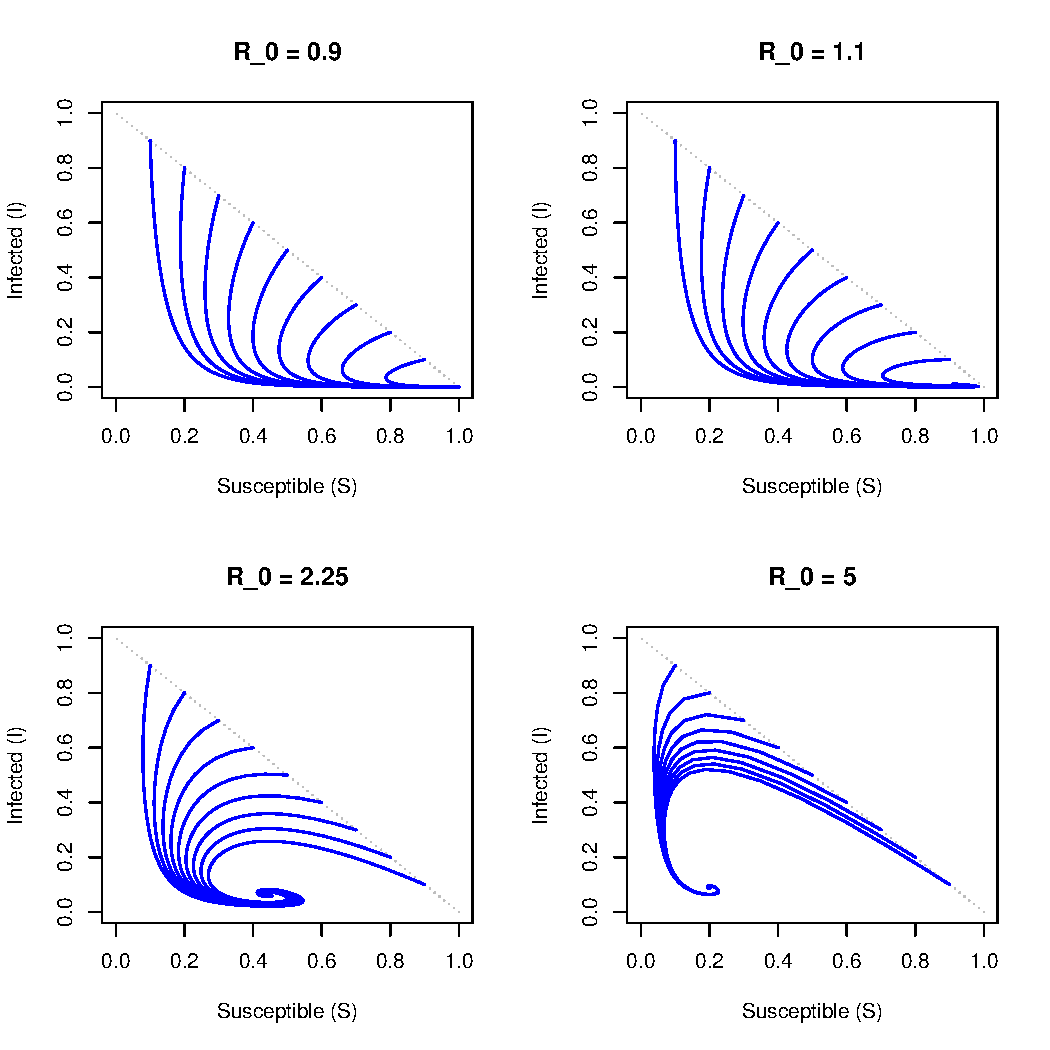
\includegraphics[width=6cm]{figure/phase_portraits-1} 
\includegraphics[width=6cm]{figure/phase_portraits-2} 
\includegraphics[width=6cm]{figure/phase_portraits-3} 
\includegraphics[width=6cm]{figure/phase_portraits-4} 

}

\caption{\label{fig:phase.portraits} Phase portraits for a single patch and various treatment models. Parameters are $\mu=0.15,\ \beta_i=0.06,\ \gamma=0.14,\ \sigma=0.07,\ \beta_w=0.15,\ \xi=10,\ \rho=0.9,\ \nu=0.9,\ \eta=0.9,\ \alpha=0$. The initial conditions for the model were $S_0=0.95,\ I_0=0.05,\ R_0=0$}\label{fig:phase.portraits}
\end{figure}


\end{knitrout}

\FloatBarrier

From the phase portraits in figure \ref{fig:phase.portraits}, and the time series in figure \ref{fig:num.sim} it is clear that all treatments appear to have an effect on transmission dynamics, causing the infection to peak at a much higher level of incidence much quicker than without the treatment.
However the infectives also appear to recover comparably quickly as well, as seen by the sharp drop off in $I$.
All treatments appear to show very similar effects for the single patch model, but how work in the spatial model may differ, espescially singe the treatments can be applied heterogenously across the patches, in proportion to the initial infectives of each patch.

We hope to compare the effectiveness of these methods by comparing the final size, which can be computed from ${\mathcal R_0}$ in $R$ using Lambert's $W$ function, as noted in the supplementary material of \cite{link20}.
\begin{linenomath}
\begin{equation}
    Z({\mathcal R_0}) = 1+\frac{1}{{\mathcal R_0}}W(-{\mathcal R_0}e^{{\mathcal R_0}})
\end{equation}
\end{linenomath}
If similar final sizes are estimated for multiple treatment strategies, then relative costs of the treatments may be compared to decide between them.
Cost is not necessairily only monetary, as risk is associted with overuse of antibiotics, water sanitation requires maintenance, all strategies require work from various healthcare or engineering professions.
Further work and research needs to be done to define a more formal, specific cost comparison scheme in this case.
%Further peak prevelance can estimated from the initial conditions $S_0,I_0$ and ${\mathcal R_0}$ from following expression

\subsection{Treatment Model Discussion}
 %Why should you implement a treatment over another
  %cost analysis (?) bit; realistic implementation depending on the country\
When comparing the treatments solely based on $\mathcal R_0$ and the final size, it easy to overlook the practicality of each treatment. WASH intervention is the simplest treatment technique, with hygiene and clean water distribution usually the first treatment implementation at the start of an outbreak. 
Chlorination techniques have had a few pitfalls depending on the quality of implementation. 
Well chlorination with liquid bleach which was used during the 2008 cholera outbreak in Guinea Bissau was considered ineffective in maintaining the recommended free residual cholorine amount, whereas the use of chlorinators (slow releasing chlorine tablets) depends on the maintenance by surrounding citizens\link{link27}.
In terms of pragmatism, it is impractical to only implement antibiotic prophylaxis to those who are infected as well as those who come in contact with the with the contaminated water source (since mass antibiotic implementation would increase the chance of selecting antibiotic resistant strains) \citep{link23}. 




%End Note

\bigskip\vfill
\centerline{\bf--- END OF PROJECT---}
\bigskip
Compile time for this document:
\today\ @ \thistime\\
CPU time to generate this document: 2.038S seconds.
\printbibliography
\end{document}
